\chapter{Quantization}

As mentioned in the introduction, two operations are necessary to transform an analog waveform into a digital signal.
The first action, discussed in Chapter~\ref{chapter:FourierAnalysisSampling}, is called sampling.
It consists of converting a continuous-time input into a discrete-time signal.
The second operation is the process of approximating continuous-space samples by a discrete set of possible symbols.
This process termed \emph{quantization} is equally essential in order to transmit an analog signal over digital media.
Quantization invariably induces a loss in signal quality.
The \emph{distortion} between the original and quantized signals is usually unwanted, and cannot be reversed.
Yet, for a specific application, the level of signal degradation can be controlled.


\section{Scalar Quantizers}

Generic quantizers operate on large classes of signals and are very robust.
In scalar quantization, each source value is processed individually, with the quantizer output taking one of finitely many possibilities.
The number of quantization levels tends to be a base-two exponent because the output of the quantizer is often represented using binary symbols.
Mathematically, a quantizer can be expressed as a function.
Suppose that the input to the quantizer is a real number, and its output is a value that belongs to the set $\mathcal{Q}$.
Then we can describe the quantizer as a function $Q : \mathbb{R} \mapsto \mathcal{Q}$ with output
\begin{equation*}
x_{\mathrm{q}} = Q(x) .
\end{equation*}
This is perhaps best seen through an example.


\begin{example}
Let $Q : \mathbb{R} \mapsto \mathcal{Q}$ be a quantizer with four possible outputs labeled $q_1$ through $q_4$.
The output $x_{\mathrm{q}}$ of the quantizer belongs to set $\mathcal{Q}$, and it must therefore be equal to one of the four possible points listed above.
Figure~\ref{figure:Quantizer} shows the functional representation of a four-level quantization scheme.
\begin{figure}[htbp]
\begin{center}
\begin{psfrags}
\psfrag{q1}[l]{$q_1$}
\psfrag{q2}[l]{$q_2$}
\psfrag{q3}[l]{$q_3$}
\psfrag{q4}[l]{$q_4$}
\psfrag{o}[c]{Output}
\psfrag{i}[c]{Input}
\epsfig{file=Figures/quantizer,width=6cm}
\end{psfrags}
\caption{A functional representation of a quantizer.}
\label{figure:Quantizer}
\end{center}
\end{figure}

The output of the quantizer in this example is determined according to a nearest neighbor rule.
Note that this function is not injective (one-to-one) and, as such, has no inverse.
\end{example}


\section{Distortion Measures}

To compare different quantizers, a performance metric must be established.
A common distortion criterion with nice properties is the square of the error
\begin{equation} \label{equation:QuantizationErrorSquared}
d(x, x_{\mathrm{q}}) = (x - Q(x))^2 = e_{\mathrm{q}}^2 ,
\end{equation}
where $e_{\mathrm{q}} = x - x_{\mathrm{q}}$ is the \emph{quantization error}.
The criterion in \eqref{equation:QuantizationErrorSquared} specifies how close the output $x_{\mathrm{q}}$ is to $x$ for a specific realization of $x$.
Since the quantizer is designed to operate on an information signal, a more relevant assessment of performance weighs in the accuracy of the quantizer over all possible realizations of the input.
An appropriate distortion measure for the quantization of a random signal is provided by the \emph{mean squared error (MSE)},
\begin{equation} \label{equation:QuantizationMSE}
\mathrm{E} [ d(x, x_{\mathrm{q}}) ]
= \mathrm{E} \left[ (x - Q(x))^2 \right] = \| e_{\mathrm{q}} \|^2 .
\end{equation}
Note that this performance metric depends on the distribution of the input signal, and hence is tied to a specific application.
A quantizer can be said to work well in a particular context.
However, describing the performance of a quantization scheme without specifying the properties of its input signal is meaningless.

\begin{example} \label{example:UniformQuantizer}
Suppose that the values of a discrete-time information signal are uniformly distributed over $[0,16]$.
Furthermore, assume that the quantizer implements a nearest neighbor rule with quantization levels equal to $q_i = 2i - 1$ for $i = 1, 2, \ldots, 8$.
We wish to find the mean squared error of this quantization scheme.

Being uniformly distributed, the probability density function of the input signal is
\begin{equation*}
f_x (\xi) = \frac{1}{16}
\end{equation*}
for $\xi \in [0, 16]$, and zero otherwise.
The decision regions corresponding to the various quantization points are then given by $[0, 2], (2, 4], \ldots, (14, 16]$.
We can therefore compute the mean squared error as follows,
\begin{equation*}
\begin{split}
\mathrm{E} [ d(x, x_{\mathrm{q}}) ]
&= \mathrm{E} \left[ (x - Q(x))^2 \right]
= \int_0^{16} \frac{(\xi - Q(\xi))^2}{16} d\xi \\
&= \sum_{i=1}^8 \int_{2i-2}^{2i} \frac{(\xi - (2i - 1))^2}{16} d\xi \\
&= \frac{1}{2} \int_{0}^{2} (\xi + 1)^2 d\xi = \frac{1}{3} .
\end{split}
\end{equation*}
That is, the mean square error associated with this input distribution and quantization scheme is $\| e_{\mathrm{q}} \|^2 = \frac{1}{3}$.
\end{example}

One of the criticisms about the MSE of \eqref{equation:QuantizationMSE} is that it has a tendency to assign a larger distortion value to signal input with sizable second moments.
Indeed, an information process likely to feature large amplitudes is bound to yield outputs with a large mean squared error.
On the other hand, under this absolute metric, most quantizers may appear to work well for minute signals as their mean square errors are destined to remain small.
An alternative and closely related criterion that takes into consideration the power of the original signal is the \emph{signal-to-quantization-noise ratio (SQNR)},
\begin{equation} \label{equation:SQNR}
\text{SQNR} = \frac{\| x \|^2}{\| e_{\mathrm{q}} \|^2}
= \frac{\mathrm{E} \left[ x^2 \right]}{\mathrm{E} \left[ (x - Q(x))^2 \right]} .
\end{equation}
Because of the implicit normalization associated with \eqref{equation:SQNR}, this latter performance measure is more suitable to compare quantizer performance for different input processes.

\begin{example}
This time, assume that the values of a discrete-time information signal are uniformly distributed over $[0,2]$.
To avoid confusion, we denote the input signal in the present problem using $y$.
We wish to obtain the mean squared error associated with the quantizer of Example~\ref{example:UniformQuantizer}, applied to the signal at hand.
Also, we wish to compare the SQNR of the quantization scheme of Example~\ref{example:UniformQuantizer} with the SQNR of the scenario described in this example.

To derive the mean squared error, we follow the same steps as before
\begin{equation*}
\begin{split}
\mathrm{E} [ d(y, y_{\mathrm{q}}) ]
&= \int_0^{2} \frac{(\zeta - Q(\zeta))^2}{2} d\zeta \\
&= \frac{1}{2} \int_{0}^{2} (\zeta - 1)^2 d\zeta = \frac{1}{3} .
\end{split}
\end{equation*}
We notice that the MSE is the same as the one derived in Example~\ref{example:UniformQuantizer}.
Nevertheless, the quantization scheme seems more suited to the signal described in the previous example.
The SQNR of the current scheme is given by
\begin{equation*}
\text{SQNR} = \frac{\| y \|^2}{\mathrm{E} [ d(y, y_{\mathrm{q}}) ]}
= 3 \| y \|^2 = 4.
\end{equation*}
This can be compared with the SQNR of the problem featured in Example~\ref{example:UniformQuantizer}, which is given by
\begin{equation} \label{equation:UniformQuantizerSQNR}
\text{SQNR} = \frac{\| x \|^2}{\mathrm{E} [ d(x, x_{\mathrm{q}}) ]}
= 3 \| x \|^2 = 256.
\end{equation}
Obviously, the SQNR is much better in the case of Example~\ref{example:UniformQuantizer}.
Can you think of an eight-level quantization scheme that would perform better for the current problem, perhaps rivaling the SQNR of \eqref{equation:UniformQuantizerSQNR}?
\end{example}

Both the mean squared error and the signal-to-quantization-noise ratio are valid and meaningful ways to present performance results for quantization schemes.
Still, they must be put in proper context, especially when comparing scenarios where the distributions of the input signals differ.
For a fixed input process, a quantization scheme that minimizes the MSE will invariably maximize the SQNR.


\section{Uniform Quantizers}
\label{section:UniformQuantizers}

Finding an optimal quantizer is not an easy task.
An eight-level quantizer has eight degrees of freedom, and the overall performance of the quantizer is jointly determined by the positions of the quantization points.
A means to reduce the difficulty of identifying an optimal quantization scheme is to constraint the possible candidates.
This can be achieved, for instance, by imposing a rule on the respective position of the quantization points.
Restricting the search space to uniform quantizers is one possible way to ensure that an optimal quantizer can be found.

A \emph{uniform quantizer} is a function where the locations of successive outputs are situated at a fixed interval, $q_i - q_{i-1} = \Delta$ for all the possible values.
That is, the distance between two quantization points is the same for all neighbors.
This scheme is one of the simplest quantizer designs.
The quantization function considered in Figure~\ref{figure:Quantizer} is in fact a uniform quantizer.
If the objective function of the optimization process is the mean squared error, then optimal locations for the quantization points can be found in a straightforward manner.
First, note that we can write the position of the quantization points as
\begin{equation*}
q_i = q_1 + (i-1) \Delta
\end{equation*}
for $i = 1, 2, \ldots, \ell$ where $\ell$ is the number quantization levels.
As usual, the MSE is given by
\begin{equation*}
\mathrm{E} [ d(x, x_{\mathrm{q}}) ]
= \int_{-\infty}^{\infty} (\xi - Q(\xi))^2 f_x(\xi) d\xi .
\end{equation*}
We emphasize  that the performance of the quantizer is optimize by minimizing the value of the integrant at each point.
We deduce that the decision regions corresponding to $q_1, q_2, \ldots, q_{\ell}$ must be equal to
\begin{equation*}
\left( - \infty, q_1 + \frac{\Delta}{2} \right],
\left( q_2 - \frac{\Delta}{2}, q_2 + \frac{\Delta}{2} \right],
\ldots,
\left( q_{\ell} - \frac{\Delta}{2}, \infty \right) ,
\end{equation*}
respectively.
The objective function then becomes
\begin{equation} \label{equation:UniformQuantizerMSE}
\begin{split}
\text{MSE} &= \int_{-\infty}^{q_1 + \frac{\Delta}{2}} (\xi - q_1)^2 f_x(\xi) d\xi
+ \sum_{i=2}^{{\ell}-1}
\int_{q_i - \frac{\Delta}{2}}^{q_i + \frac{\Delta}{2}}
(\xi - q_i)^2 f_x(\xi) d\xi \\
&+ \int_{q_{\ell} - \frac{\Delta}{2}}^{\infty} (\xi - q_{\ell})^2 f_x(\xi) d\xi .
\end{split}
\end{equation}
The resulting optimization process now has two degrees of freedom, namely $q_1$ and $\Delta$.
For a suitable probability density function $f_x(\cdot)$, an optimal solution can be obtained explicitly using standard optimization methods.

\begin{example} \label{example:OptimalUniformQuantizer}
We revisit Example~\ref{example:UniformQuantizer} in the context of uniform quantizers.
Again, suppose that the values of the discrete-time input process are uniformly distributed over $[0, 16]$.
We wish to find the optimal eight-level uniform quantizer associated with this input distribution.

For simplicity, we assume that the quantization points $\{ q_1, q_2, \ldots, q_8 \}$ are contained in the interval $[0, 16]$.
This implies that $q_1 > 0$ and $q_8 < 16$.
The mean squared error as a function of $q_1$ and $\Delta$ is given by \eqref{equation:UniformQuantizerMSE}, which becomes
\begin{equation*}
\begin{split}
\text{MSE}~(q_1, \Delta)
%&= \int_{0}^{q_1 + \frac{\Delta}{2}} \frac{(\xi - q_1)^2}{16} d\xi
%+ \sum_{i=2}^{7}
%\int_{q_i - \frac{\Delta}{2}}^{q_i + \frac{\Delta}{2}}
%\frac{(\xi - q_i)^2}{16} d\xi
%+ \int_{q_8 - \frac{\Delta}{2}}^{16} \frac{(\xi - q_8)^2}{16} d\xi \\
&= \int_{-q_1}^{\frac{\Delta}{2}} \frac{\xi^2}{16} d\xi
+ 6 \int_{- \frac{\Delta}{2}}^{\frac{\Delta}{2}} \frac{\xi^2}{16} d\xi
+ \int_{- \frac{\Delta}{2}}^{16 - q_8} \frac{\xi^2}{16} d\xi \\
\end{split}
\end{equation*}
Recall that, by construction, we can write $q_8 = q_1 + 7 \Delta$.
Taking first derivatives with respect to $q_1$ and $\Delta$, we obtain
\begin{align*}
\frac{\partial}{\partial q_1} \text{MSE}~(q_1, \Delta)
&= \frac{q_1^2}{16} - \frac{(16 - q_1 - 7 \Delta)^2}{16} \\
\frac{\partial}{\partial \Delta} \text{MSE}~(q_1, \Delta)
&= \frac{7 \Delta^2}{64} - \frac{7 (16 - q_1 - 7\Delta)^2}{16} .
\end{align*}
Setting these derivatives equal to zero, we get $q_1 = 1$ and $\Delta = 2$.
A second derivative test ensures that this corresponds to a local minimum.
Since this point is the only stationary point of the function $\text{MSE}~(q_1, \Delta)$ within our search space, we gather that the quantization scheme of Example~\ref{example:UniformQuantizer} coincide with the optimal uniform quantizer.
\end{example}

Although the search space for uniform quantizers is much smaller than the set of all possible quantizers, finding an optimal uniform quantizer remains a strenuous task in most situations.
The resulting minimization problem need not have a closed-form solution, in contrast to Example~\ref{example:OptimalUniformQuantizer}.
This task is often accomplished by discretizing the search space and applying numerical techniques to identify the best candidate.


\section{Non-Uniform Quantizers}
\label{section:NonUniformQuantizers}

For a \emph{non-uniform quantizer}, the restriction that neighboring quantization points should be equidistant from one another is removed.
As such, these points can be located anywhere on the real line, and the decision region corresponding to each quantization point need not have a simple structure.
The collection of non-uniform quantizers is much larger then the set of uniform quantizers described in Section~\ref{section:UniformQuantizers}.
This greater flexibility in choosing a quantizer often results in better overall performance.
However, it also comes with added complexity in designing the quantization scheme.
In this section, we explore some properties of an optimal quantizer for the mean squared error criterion and we present an algorithm that can be employed to obtain a non-uniform quantizer.

First, suppose that the quantization points $\{ q_i \}$ are fixed.
An optimal quantizer for these points is a function $Q^* : \mathbb{R} \mapsto \mathcal{Q}$ that minimizes the corresponding MSE,
\begin{equation*}
\begin{split}
\min_Q \mathrm{E} [ d(x, x_{\mathrm{q}}) ]
&= \min_Q \int_{-\infty}^{\infty} (\xi - Q(\xi))^2 f_x(\xi) d\xi \\
&= \int_{-\infty}^{\infty} \min_{Q(\xi)} (\xi - Q(\xi))^2 f_x(\xi) d\xi .
\end{split}
\end{equation*}
The last equality follows from the fact that a quantization point can be selected independently for every possible input value.
It should then be clear that the value of the function $Q^*(\cdot)$ evaluated at $x$ is the point $q_i$ that is closest to $x$,
\begin{equation*}
Q^*(x) = \arg \min_{\{ q_i \}} (x - q_i)^2 .
\end{equation*}
In particular, an optimal $\ell$-level scalar quantizer always has $\ell$ decision regions, each being an interval containing its quantization point.

Alternatively, we can assume that the decision intervals are given.
Let the boundaries of these intervals be denoted by $b_1, b_2, \ldots, b_{\ell-1}$.
Then, the corresponding MSE is given by
\begin{equation} \label{equation:BoundaryQuantizationMSE}
\int_{-\infty}^{b_1} (\xi - q_1)^2 f_x(\xi) d\xi
+ \sum_{i=2}^{{\ell}-1}
\int_{b_{i-1}}^{b_i} (\xi - q_i)^2 f_x(\xi) d\xi
+ \int_{b_{\ell-1}}^{\infty} (\xi - q_{\ell})^2 f_x(\xi) d\xi .
\end{equation}
The value of the MSE can be minimized by selecting the quantization points $\{ q_i \}$ appropriately.
Note that each quantization point can be optimized individually, as the integrals in \eqref{equation:BoundaryQuantizationMSE} have a nice additive structure.
Solving one instance of the decouple problem, we get
\begin{equation*}
q_i^* = \min_{q_i} \int_{b_{i-1}}^{b_i} (\xi - q_i)^2 f_x(\xi) d\xi .
\end{equation*}
To obtain the solution, we differentiate the objective function with respect to $q_i$ and set the derivative equal to zero;
\begin{equation*}
\frac{d}{d q_i} \int_{b_{i-1}}^{b_i} (\xi - q_i)^2 f_x(\xi) d\xi
= \int_{b_{i-1}}^{b_i} 2 (\xi - q_i) f_x(\xi) d\xi = 0 .
\end{equation*}
This implies that
\begin{equation*}
q_i^* = \mathrm{E} [ x | b_{i-1} < x \leq b_i ] .
\end{equation*}
Once the decision intervals are picked, the optimal quantization point $q_i^*$ is equal to the expectation of $x$ conditioned on $x$ falling inside interval~$i$.

Putting these two observations together, we can summarized the properties of an optimal $\ell$-level quantizer as follows.
Suppose that $Q^* : \mathbb{R} \mapsto \mathcal{Q}$ is an optimal quantizer with respect to the mean square error criterion (or the signal-to-quantization-noise ratio).
Then, the decision regions corresponding to the quantization points $\{ q_i \}$ form a partition of the real line where each decision set is an interval.
Given the positions of the various quantization points $\{ q_i \}$, the boundaries of the decision intervals are given by
\begin{equation*}
b_i = \frac{q_i + q_{i+1}}{2}
\end{equation*}
where $i = 1, 2, \ldots, \ell-1$.
Furthermore, the quantization point corresponding to decision interval $(b_{i-1}, b_i]$ is equal to the expectation of $x$ conditioned on $b_{i-1} < x \leq b_i$.
These properties are collectively known as the \emph{Lloyd-Max} conditions.


\subsection{Lloyd-Max Algorithm}

The Lloyd-Max conditions enumerated above form a set of rules that are necessarily fulfilled by optimal quantizers.
Yet, they do not provide an explicit means to compute the exact positions of the quantization points in an optimal quantizer.
Furthermore, it may not be possible to find these points analytically.

A method that is frequently used to find a non-uniform scalar quantizer is the \emph{Lloyd-Max algorithm}.
This algorithm starts with an initial assignment for the quantization points which, in this case, we label $q_1^{(0)}, q_2^{(0)}, \ldots, q_{\ell}^{(0)}$.
The ensuring procedure is to alternate iteratively between the following two steps.
\begin{enumerate}
\item Compute the boundaries of the decision intervals according to
\begin{equation*}
b_i^{(t)} = \frac{q_i^{(t)} + q_{i+1}^{(t)}}{2} , \quad 
i = 1, 2, \ldots, \ell - 1 .
\end{equation*}
\item Find the updated values of the quantization points,
\begin{equation*}
q_i^{(t+1)} = \mathrm{E} [x | b_{i-1} < x \leq b_i ] , \quad
i = 1, 2, \ldots, \ell .
\end{equation*}
\end{enumerate}
We adopt the simplifying notation $b_0 = - \infty$ and $b_{\ell} = \infty$ to express the conditional expectation in a consistent manner.
The MSE of the quantization scheme decreases at every step, thereby becoming smaller than the MSE of all the previous assignments.
This insures that performance improves with every iteration.
The algorithm terminates when a satisfactory level of performance has been achieved, or when the quantization points have converged to their final values.
% While the Lloyd-Max algorithm typically leads good quantizers, it is not guaranteed to converge to the optimal solution.


\section{Vector Quantizers}

A quantizer can work either on single-source outputs or on blocks of source outputs.
So far, we have studied the former approach by focusing on scalar quantizers.
Although more involved, the second method where multiple outputs are aggregated prior to being quantized typically yields better results.
This latter approach, called \emph{vector quantization}, is especially powerful for sources producing signals that are strongly correlated over time.
We do not explore the details of vector quantization in this document, however we motivate it purpose through a simple example.

\begin{example} \label{example:VectorQuantization}
Assume that a source produces two correlated symbols, denoted $x$ and $y$.
We are tasked with designing a vector quantizer for this source with a total of four quantization points.
The joint probability distribution function associated with this source is known to be
\begin{equation} \label{equation:QuantizationJointPDF}
\begin{split}
f_{x,y} (\xi, \zeta) &= \frac{1}{4} g ( \xi + 1.5, \zeta + 1.5 )
+ \frac{1}{4} g ( \xi + 0.5, \zeta + 0.5 ) \\
&+ \frac{1}{4} g ( \xi - 0.5, \zeta - 0.5 )
+ \frac{1}{4} g ( \xi - 1.5, \zeta - 1.5 ) ,
\end{split}
\end{equation}
where the function $g(\cdot, \cdot)$ is given by
\begin{equation*}
g(\xi, \zeta) = \begin{cases} 1, &  |\xi|, |\zeta| < 0.5 \\
0, & \text{otherwise}. \end{cases}
\end{equation*}
For illustrative purposes, $f_{x,y} (\cdot, \cdot)$ is shown in Figure~\ref{figure:VectorQuantization}.
\begin{figure}[htbp]
\begin{center}
\begin{psfrags}
\psfrag{x}[c]{$x$}
\psfrag{y}[c]{$y$}
\psfrag{f}[l]{$f_{x,y}(\cdot, \cdot)$}
\epsfig{file=Figures/vectorquantization,width=6cm}
\end{psfrags}
\caption{A graphical rendering of the joint probability density function defined in \eqref{equation:QuantizationJointPDF}.}
\label{figure:VectorQuantization}
\end{center}
\end{figure}
The four quantization points for the vector quantizer are located at $q_1 = (-1.5, -1.5)$, $q_2 = (-0.5, -0.5)$, $q_3 = (0.5, 0.5)$, and $q_4 = (1.5, 1.5)$.
The MSE associated with our vector quantizer can therefore be computed as
\begin{equation*}
\begin{split}
&\mathrm{E} \left[ \| (x,y) - Q(x,y) \|^2 \right] \\
&= \int_{-\infty}^{\infty} \int_{-\infty}^{\infty}
\| (\xi, \zeta) - Q(\xi, \zeta) \|^2 f_{x,y}(\xi,\zeta) d\xi d\zeta \\
&= 4 \int_{-0.5}^{0.5} \int_{-0.5}^{0.5} \frac{\xi^2 + \zeta^2}{4} d\xi d\zeta
= \frac{1}{6} .
\end{split}
\end{equation*}
That is, the MSE per pair of symbols associated with our vector quantizer is $\frac{1}{6}$.
Note that we have used an extended version of the mean squared error that accounts for the 2-D aspect of the problem.

Suppose instead that we wish to use an optimal scalar quantizer instead of the aforementioned vector quantizer.
We are then left with two quantization points per axis.
The marginal distributions of the source symbols are given by
\begin{equation*}
f_x (\varphi) = f_y (\varphi)
= \begin{cases} \frac{1}{4}, & |\varphi| < 2 \\
0, & \text{otherwise} . \end{cases}
\end{equation*}
The optimal scalar quantization scheme in this case is to put one point at $-1$ and the other at $1$.
Once combined, the two scalar quantizers are equivalent to having points at $\tilde{q}_1 = (1,1)$, $\tilde{q}_2 = (-1,1)$, $\tilde{q}_3 = (-1,-1)$, and $\tilde{q}_4 = (1,-1)$ in the plane.
The resulting MSE per pair of symbols becomes
\begin{equation*}
\begin{split}
&\mathrm{E} \left[ \left\| (x,y) - \tilde{Q}(x,y) \right\|^2 \right] \\
&= \int_{-\infty}^{\infty} \int_{-\infty}^{\infty}
\left\| (\xi, \zeta) - \tilde{Q}(\xi, \zeta) \right\|^2 f_{x,y}(\xi,\zeta) d\xi d\zeta \\
&= 4 \int_0^1 \int_0^1 \frac{\xi^2 + \zeta^2}{4} d\xi d\zeta
= \frac{2}{3} .
\end{split}
\end{equation*}
Comparing with our previous result, we notice that the MSE is much larger when using the scalar approach.
\begin{figure}[htbp]
\begin{center}
\begin{psfrags}
\psfrag{q1}[l]{$q_1$}
\psfrag{q2}[l]{$q_2$}
\psfrag{q3}[l]{$q_3$}
\psfrag{q4}[l]{$q_4$}
\psfrag{s1}[l]{$\tilde{q}_1$}
\psfrag{s2}[l]{$\tilde{q}_2$}
\psfrag{s3}[l]{$\tilde{q}_3$}
\psfrag{s4}[l]{$\tilde{q}_4$}
\psfrag{x}[c]{$x$}
\psfrag{y}[c]{$y$}
\epsfig{file=Figures/vectorquantizer,width=6cm}
\end{psfrags}
\caption{A visual graphical comparison of vector and scalar quantization schemes applied to the two-dimensional problem of Example~\ref{example:VectorQuantization}.}
\label{figure:VectorQuantizer}
\end{center}
\end{figure}
\end{example}

Although this example may not be the most realistic scenario, it provides a good illustration of the potential benefits associated with using vector quantizers.
The improved performance comes from the greater flexibility in positioning the various quantization points in a high-dimensional setting together with the ability to exploit correlation among consecutive source symbols.
On the downside, the mathematical treatment of a quantization problem becomes more intricate in a higher-dimensional space.


\section{Analysis-Synthesis Algorithms}

All the quantizers described up to this point are generic schemes designed to work well with abstract sources.
In practice, many quantization algorithms are tailored to a specific applications.
These quantizers are called \emph{analysis-synthesis} coders, and their design is typically fairly intricate.
They require advanced models and are often evaluated according to complex performance metrics.
These criteria are rooted in human perception rather than conventional mathematics.
When developed properly, model-based quantization schemes achieve better compression ratios than the \emph{waveform coders} presented until now.
A serious treatment of analysis-synthesis algorithms is beyond the scope of this document.
Nevertheless, we mention two popular schemes below for illustrative purposes.

\paragraph{Speech Coding:}
The quantization mechanism employed in speech coding provides a nice example of an analysis-synthesis scheme.
Speech coders are widely used in mobile telephony and VoIP.
Human speech is modeled as a much simpler random process than most other audio signals, and there is an abundance of knowledge about its statistical properties and the way voice is generated.
As a result, some auditory information which is relevant in generic audio signals becomes inconsequential in the context of speech.
The primary performance criteria for voice signals are intelligibility and pleasantness of the received signal.
In addition, most speech applications require low delay, as long delays interfere with speech interaction in real-time applications.
The \emph{Code Excited Linear Prediction (CELP)} is a class of algorithms developed for human speech.
The basic idea behind this approach is to model human speech production using a time-varying linear filter.
The speech samples are subsequently separated in two distinct parts.
The first component contains the current parameters governing the operation of the linear filter; these parameters are selected from a finite set of possible values.
The second component captures the residual error, the difference between the predicted signal and the actual one.
This second signal is quantized using standard waveform coding techniques.
The overall operation of the system works quite well for conversations.
However, a speech coder applied to music fails to provide an adequate rendition of the original signal.

\paragraph{Joint Photographic Experts Group (JPEG):}
The JPEG algorithm is a file format designed to store photographs and paintings digitally.
The acronym JPEG is derived from the name of the committee that created this standard.
A JPEG file can actually be created in various ways.
A commonly used procedure specified in this standard is the \emph{JPEG file interchange format (JFIF)}, which we describe briefly.
The encoding process consists of several steps.
First, an image is represented using YCbCr, an encoding scheme that specifies every pixel (sample point) in the image according to a light intensity component (Y) and two chroma (Cb and Cr) for colors.
This scheme, as opposed to RGB, is interesting because it parallels the way the human visual system perceives image elements.
The image is then split into blocks of $8 \times 8$ pixels; and for each block, the Y, Cb, and Cr data undergoes a two-dimensional cosine transform.
This step is similar to a Fourier transform in the sense that it produces a spatial frequency spectrum.
The amplitudes of the resulting frequency components are quantized.
The resolution of the chroma data is reduced, compared to the light intensity component.
This reflects the fact that the human eye is less sensitive to fine color details than to fine brightness details.
Furthermore, human perception is much more sensitive to small variations in color or brightness over large areas than to the strength of high-frequency brightness variations.
Thus, the magnitudes of the high-frequency components are stored with a lower accuracy than the low-frequency components.
The resulting data for all $8 \times 8$ blocks is further compressed with a lossless algorithm, a variant of \emph{Huffman encoding}.
The important concept exposed in this example is how JPEG is built with a specific application in mind, and therefore quantizes sample data as to minimize the perceived distortion.
This is a very good illustration of an analysis-synthesis quantizer.


